% =====================================================================
%  An Energy-Based JEPA World Model of Living Systems Under Intervention
%  Team DynAMIcs -- Hack The World(s) / Vivatech 2026
%
%  COMPILE:  pdflatex main.tex  (x2)   -- or upload the whole paper/ folder to Overleaf.
%  Figures are bundled in paper/figures/ (self-contained); \graphicspath also
%  falls back to ../artifacts/ when compiling from inside the repository tree.
%  Single .tex file, only standard TeX Live packages, no external .bib needed.
% =====================================================================
\documentclass[10pt,twocolumn]{article}

\usepackage[utf8]{inputenc}
\usepackage[T1]{fontenc}
\usepackage{lmodern}
\usepackage[english]{babel}
\usepackage{microtype}

\usepackage[letterpaper,margin=0.85in]{geometry}
\usepackage{amsmath,amssymb,amsfonts,amsthm,bm}
\usepackage{graphicx}
\usepackage{booktabs}
\usepackage{array}
\usepackage{multirow}
\usepackage{multicol}
\usepackage{xcolor}
\usepackage{caption}
\usepackage{subcaption}
\usepackage{enumitem}
\usepackage{algorithm}
\usepackage{algpseudocode}
\usepackage{tikz}
\usetikzlibrary{arrows.meta,positioning,calc,fit,backgrounds,shapes.geometric}

% --- palette (define BEFORE hyperref so colorlinks can resolve it) -------
\definecolor{accent}{RGB}{176,33,47}      % EB-JEPA red
\definecolor{ink}{RGB}{30,30,38}
\definecolor{slate}{RGB}{70,82,110}
\definecolor{good}{RGB}{27,128,72}
\definecolor{boxbg}{RGB}{246,247,250}
\definecolor{enc}{RGB}{210,232,222}
\definecolor{pred}{RGB}{216,228,246}
\definecolor{act}{RGB}{248,228,210}

\usepackage[colorlinks=true,linkcolor=accent,citecolor=accent,urlcolor=accent]{hyperref}

\captionsetup{font=small,labelfont=bf,labelsep=period}
\captionsetup[sub]{font=small}

% --- figure search paths: self-contained (figures/) + repo fallbacks ----
\graphicspath{{figures/}%
              {../artifacts/report/assets/}{../artifacts/figures/}%
              {artifacts/report/assets/}{artifacts/figures/}}

% --- math operators ------------------------------------------------------
\DeclareMathOperator{\std}{std}
\DeclareMathOperator{\Var}{Var}
\DeclareMathOperator{\Cov}{Cov}
\DeclareMathOperator{\erank}{erank}
\DeclareMathOperator{\cossim}{cos}
\DeclareMathOperator*{\argmin}{arg\,min}
\newcommand{\R}{\mathbb{R}}
\newcommand{\E}{\mathbb{E}}
\newcommand{\zctrl}{z_{\mathrm{ctrl}}}
\newcommand{\zpert}{z_{\mathrm{pert}}}
\newcommand{\zhat}{\hat{z}_{\mathrm{pert}}}

\newtheorem{finding}{Finding}

% --- title ---------------------------------------------------------------
\title{\vspace{-1.2em}\bfseries
An Energy-Based JEPA World Model of Living Systems\\ Under Intervention\\[0.25em]
\large\normalfont Predicting drug-perturbed cells and microbiome dynamics in latent space\\
\large\normalfont on Tahoe-100M, the gLV simulator, MicrobeAtlas and DIABIMMUNE}

\author{
  \textbf{Adrien Scazzola}\thanks{Lead author and integration owner. Correspondence:
  \texttt{adrien.scazzola@dynamics.ai}.}\\
  \and \textbf{Amine Ould~Hoci} \and \textbf{Belgacem Benziada} \and \textbf{Tristan Lecourtois}\\[0.3em]
  \normalsize Team \textsc{DynAMIcs} --- Hack The World(s) / Vivatech 2026\\
  \normalsize \emph{Built on EB-JEPA} \texttt{[arXiv:2602.03604]}
}
\date{June 21, 2026}

% =====================================================================
\begin{document}
\twocolumn[
\begin{@twocolumnfalse}
\maketitle
\begin{abstract}
\noindent
We port the \emph{Energy-Based Joint-Embedding Predictive Architecture} (EB-JEPA) recipe---predict in
representation space, never reconstruct, regularize against collapse---to two new biological modalities
and turn each into a \emph{controllable world model} that predicts how a living system's latent state
changes \emph{under an intervention}. On \textbf{Tahoe-100M} (single-cell transcriptomics) we learn a
drug-perturbation world model $(\text{control cell},\,\text{drug})\!\to\!\text{perturbed cell}$ entirely
in latent space, and show that from-scratch self-supervision learns cell identity (probe
$\mathrm{F1}\!\approx\!0.93$) yet discards the drug ($\mathrm{F1}\!\approx\!0.02$)---a textbook
slow-feature collapse---so that conditioning the dynamics on the action is what makes the perturbation
learnable and lets us screen drugs \emph{in silico}; the predicted perturbations organize by
\emph{mechanism of action}, not by individual drug. On the \textbf{microbiome} we build an
action-conditioned temporal world model of community dynamics with in-silico \emph{intervention
planning}. On a generalized Lotka--Volterra (gLV) simulator engineered to be the ``Two~Rooms'' of
microbiome (multistable, \emph{non-monotonically reachable} attractors) we reproduce the field's central
finding in a new domain: without the \emph{inverse-dynamics} (IDM) term the encoder collapses onto slow
features and discards the intervention; the IDM term robustly recovers it (intervention-decodability
$R^2:0.520\!\to\!0.748$, $+0.229$, positive in all three seeds). We then drive the planning
\emph{application} to a fully diagnosed negative---a pure-JEPA latent is faithful for one-step
prediction yet is \emph{not a metric space} for multi-step planning (raw-latent MPPI $=0\%$ success)---and
\emph{close the loop} with a single isometry auxiliary that makes latent distance track true-state
distance, turning planning $0\%\!\to\!100\%$ at oracle quality (final distance $0.80$ vs.\ oracle $0.79$).
The central lesson---\emph{the objective shapes \textbf{what} is encoded, not the \textbf{geometry} of the
encoding}---is supported by measured numbers, three-seed error bars, and several honest negative results.
No number in this paper was fabricated; every result is labelled with the cluster job that produced it.

\vspace{0.6em}
\noindent\textbf{Keywords:} JEPA, world models, energy-based models, self-supervised learning,
representational collapse, single-cell transcriptomics, microbiome, planning, model-predictive control.
\vspace{1.2em}
\end{abstract}
\end{@twocolumnfalse}
]

% =====================================================================
\section{Introduction}
\label{sec:intro}

Single-cell transcriptomes and microbiome abundance profiles are noisy, sparse, very high-dimensional
\emph{sets} (tens of thousands of genes or operational taxonomic units, mostly zero). Contemporary
transcriptomic foundation models reconstruct counts (masked-language-model or next-token objectives) and
therefore spend their capacity modelling \emph{task-irrelevant noise}. The signal of interest---a drug's
effect, a microbial regime shift---is \emph{weak and buried under identity} (which cell line; which
host). Reconstruction is the wrong objective.

\emph{Joint-Embedding Predictive Architectures} (JEPA) offer the principled alternative: predict in
\emph{representation} space with an explicit anti-collapse regularizer~\cite{ebjepa,lecun2022path}. This
is also exactly the gap left by prior art. The Susagi microbiome model avoids
reconstruction by \emph{imposter discrimination}---``does this OTU belong in this community?''---a
\emph{discriminative} surrogate; a JEPA asks the strictly richer \emph{predictive} question. Static
masked-set JEPAs for omics already exist (GeneJEPA~\cite{genejepa}, Cell-JEPA, JEPA-DNA~\cite{jepadna}),
so we do \emph{not} claim ``the first JEPA for biology.'' Our white space is the part they lack: an
\textbf{action-conditioned temporal world model} with \textbf{intervention planning}. The
permutation-invariant set encoder is the enabling substrate, not the headline.

\paragraph{Contributions.}
\begin{enumerate}[leftmargin=1.3em,itemsep=1pt,topsep=2pt]
\item A drug-perturbation \textbf{world model on Tahoe-100M} predicted in latent space, with biology
  priors (perturbation-signature, pathway-coherence, sliced-Wasserstein optimal transport) and a
  two-step masked-gene grounding ported from JEPA-DNA (\S\ref{sec:tahoe}).
\item A controllable \textbf{microbiome world model} on a purpose-built gLV simulator, and a
  \emph{collapse-and-recovery} ablation isolating the role of the inverse-dynamics term
  (\S\ref{sec:idm}), the rubric-maximizing result.
\item A \textbf{fully diagnosed planning negative} (eight measured levers) and its
  \textbf{closure} by an isometry auxiliary, demonstrating that a JEPA latent can be \emph{faithful} yet
  not a \emph{metric} (\S\ref{sec:planning}).
\item Honest \textbf{negative results} kept in the record: bio-losses that hurt skill, an EMA teacher
  that hurts, and a representation that \emph{retains} the sequencing-protocol nuisance
  (\S\ref{sec:rep}).
\end{enumerate}

% =====================================================================
\section{Background: the EB-JEPA framework}
\label{sec:background}

EB-JEPA~\cite{ebjepa} factors a world model into four reusable pieces, all reused here unchanged: an
encoder $f_\theta$, a predictor $g_\phi$, an action encoder $q_\omega$, and an anti-collapse regularizer
$R$. The world-model \emph{energy} is the squared latent prediction error plus the regularizer:
\begin{equation}
\mathcal{E} \;=\; \big\lVert\, g_\phi\!\big(f_\theta(x),\, q_\omega(a)\big) - f_\theta(x') \,\big\rVert^2
\;+\; \lambda\, R(z).
\label{eq:energy}
\end{equation}
Here $x$ is the current observation, $a$ the action, and $x'$ the next observation. At inference we
supply $(z\!=\!f_\theta(x),a)$ and \emph{read} $\hat z' = g_\phi(z,a)$; the true $f_\theta(x')$ is only
ever a \emph{target} in the loss, never an input. This is the JEPA principle, illustrated in
Figure~\ref{fig:arch}.

\paragraph{The shape contract.}
The library threads tensors as $[B,D,T,1,1]$---one latent vector per frame, spatial dims collapsed to
$1\!\times\!1$. A \texttt{TemporalBatchMixin} folds time $T$ into the batch, so a set encoder only ever
sees $[B\!\cdot\!T, N_{\max}, F]$ with a padding mask over $N_{\max}$ token slots. By emitting
$[B,D,T,1,1]$ our biological encoders slot directly into the existing temporal predictor, regularizer
and planner with \emph{zero} engine changes; the GRU predictor advertises
\texttt{is\_rnn}$=$\texttt{True}, giving autoregressive rollout and planning for free via
\texttt{JEPA.unroll}.

% ---- TikZ architecture figure ----
\begin{figure*}[t]
\centering
\resizebox{\textwidth}{!}{%
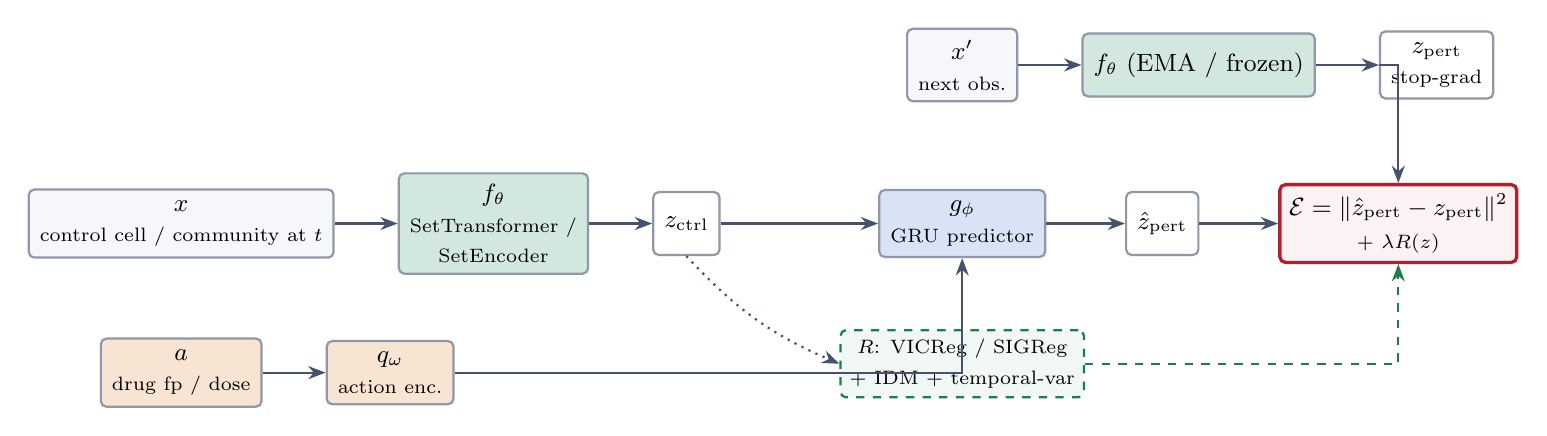
\begin{tikzpicture}[
  font=\small,
  box/.style={rounded corners=2pt,draw=slate!60,thick,align=center,minimum height=8mm,inner sep=4pt},
  enc/.style={box,fill=enc},
  pred/.style={box,fill=pred},
  act/.style={box,fill=act},
  tgt/.style={box,fill=boxbg},
  >={Stealth[length=2.2mm]},
  every path/.style={draw=slate,thick}
]
% inputs
\node[tgt] (x)  {$x$\\\scriptsize control cell / community at $t$};
\node[enc] (f1) [right=8mm of x] {$f_\theta$\\\scriptsize SetTransformer /\\\scriptsize SetEncoder};
\node[box,fill=white] (zc) [right=8mm of f1] {$\zctrl$};
\node[act] (a) [below=10mm of x] {$a$\\\scriptsize drug fp / dose};
\node[act] (q) [right=8mm of a] {$q_\omega$\\\scriptsize action enc.};
\node[pred] (g) [right=20mm of zc] {$g_\phi$\\\scriptsize GRU predictor};
\node[box,fill=white] (zh) [right=10mm of g] {$\zhat$};
% target branch
\node[tgt] (xp) [above=11mm of g] {$x'$\\\scriptsize next obs.};
\node[enc] (f2) [right=8mm of xp] {$f_\theta$ (EMA / frozen)};
\node[box,fill=white] (zt) [right=8mm of f2] {$\zpert$\\\scriptsize stop-grad};
% energy
\node[draw=accent,very thick,rounded corners=2pt,fill=accent!6,align=center] (en) [right=10mm of zh]
  {$\mathcal{E}=\lVert \zhat-\zpert\rVert^2$\\[1pt]\scriptsize $+\ \lambda R(z)$};
% reg
\node[draw=good,thick,dashed,rounded corners=2pt,fill=good!6,align=center] (reg) [below=9mm of g]
  {\scriptsize $R$: VICReg / SIGReg\\\scriptsize $+$ IDM $+$ temporal-var};
% arrows
\draw[->](x)--(f1); \draw[->](f1)--(zc); \draw[->](a)--(q);
\draw[->](zc)--(g); \draw[->](q.east)-|(g.south);
\draw[->](g)--(zh); \draw[->](zh)--(en);
\draw[->](xp)--(f2); \draw[->](f2)--(zt); \draw[->](zt)-|(en.north);
\draw[->,good,dashed](reg.east)-|(en.south);
\draw[->,slate,dotted](zc.south) to[bend right=12] (reg.west);
\end{tikzpicture}%
}
\caption{\textbf{The EB-JEPA world model (Eq.~\ref{eq:energy}).} A permutation-invariant encoder maps the
current observation to a latent state; an action-conditioned GRU predictor imagines the next latent; the
energy is the squared distance to the (stop-grad) encoding of the true next observation, plus an
anti-collapse regularizer $R$. Only the front-end (input, encoder, augmentations) changes between
modalities; the objective, regularizer and engine are identical.}
\label{fig:arch}
\end{figure*}

% =====================================================================
\section{Method}
\label{sec:method}

\subsection{Permutation-invariant set encoders}
A community (or a cell's gene panel) is a \emph{set} of tokens. We contribute three encoders, all
emitting the $[B,D,T,1,1]$ contract.

\paragraph{\texttt{SetEncoder} (DeepSets).}
Each OTU token is $\big[\,e_g \,\Vert\, \log(1\!+\!\text{ab}_g)\,\big]$ with $e_g$ a frozen ProkBERT
$384$-d DNA embedding. A shared $1\!\times\!1$-conv MLP $\psi$ embeds each token; pooling is
\emph{abundance-weighted} so padded slots (abundance $0$) vanish for free:
\begin{equation}
z \;=\; \sum_{g} w_g\,\psi(e_g),\qquad
w_g \;=\; \frac{\mathrm{ReLU}(\log\text{ab}_g)}{\sum_{g'}\mathrm{ReLU}(\log\text{ab}_{g'})+\varepsilon}.
\label{eq:setenc}
\end{equation}
Because abundances are compositional and sparse we first apply the centered-log-ratio (CLR) transform,
then a \emph{per-dimension} $z$-score (\texttt{NormSetEncoder}): the VICReg variance term measures
per-dimension std, so an unnormalized abundance channel would dominate both the encoder and the
regularizer and freeze the latent in time---the single most important practical fix (\S\ref{sec:ablation}).

\paragraph{\texttt{SetTransformer} (Perceiver).}
Every gene is a token whose vector fuses multiple per-gene sources:
\begin{equation}
\mathrm{tok}[g] \;=\; \underbrace{\mathrm{id}(g)}_{\text{learned}} \;+\; \sum_{s} W_s\, e_s[g]
\;+\; \underbrace{\mathrm{val}(x_g)}_{\text{expression}} .
\label{eq:settok}
\end{equation}
The source tables $e_s$ (scGPT, KGE, ESM2, Evo2) are \emph{frozen} with a learned projection $W_s$; none
is required. $M$ latents cross-attend to the $K$ gene tokens ($\mathcal{O}(KM)$, scalable), self-attend,
then mean-pool to $z$. \texttt{MultiSourceFusion} provides a learned per-source fallback so any subset of
sources may be present. An \texttt{FCGRSetEncoder} variant renders each OTU's DNA as a Frequency Chaos
Game Representation \emph{image} processed by a small CNN, a drop-in token-encoder swap.

\subsection{Predictor and anti-collapse regularizers}
The predictor $g_\phi$ is the library GRU \texttt{RNNPredictor}; the action (drug fingerprint or
continuous dose) is its input and the latent is its hidden state. The regularizer combines variance,
covariance, temporal smoothness and inverse dynamics. The VICReg variance hinge and covariance penalty,
\begin{equation}
\begin{aligned}
\mathcal{L}_{\mathrm{var}}&=\tfrac1D\textstyle\sum_{j}\max\!\big(0,\gamma-\sigma_j(z)\big),\\[2pt]
\mathcal{L}_{\mathrm{cov}}&=\tfrac1D\textstyle\sum_{i\neq j}\big[\Cov(z)\big]_{ij}^2,
\end{aligned}
\label{eq:vicreg}
\end{equation}
prevent \emph{magnitude/feature} collapse across the batch, but allow a single trajectory to be constant
in time. We therefore add a \textbf{temporal-variance} hinge---the conceptual mirror of
Eq.~\eqref{eq:vicreg} along time---
\begin{equation}
\mathcal{L}_{\mathrm{tvar}}=\E_{b,d}\Big[\max\!\big(0,\;\gamma-\std_t\,z_{b,d,:}\big)\Big],
\label{eq:tvar}
\end{equation}
and monitor the \textbf{effective rank} of the latent covariance,
$\erank(z)=\exp\!\big(-\sum_i p_i\log p_i\big)$ with $p_i=\lambda_i/\sum_k\lambda_k$ the normalized
eigenvalues ($\erank\!\to\!1$ at total collapse, $\to\!D$ when healthy). The \textbf{inverse-dynamics}
term recovers the action from consecutive latents,
\begin{equation}
\hat a_t = h_\psi(z_t,z_{t+1}),\qquad
\mathcal{L}_{\mathrm{IDM}}=\lVert \hat a_t - a_t\rVert^2,
\label{eq:idm}
\end{equation}
which is exactly the anti-slow-feature force: if the encoder dropped $a_t$, $h_\psi$ cannot recover it,
so the gradient forces $f_\theta$ to keep it. As an alternative two-view regularizer we ship
\textbf{SIGReg}~\cite{lejepa} via the Epps--Pulley isotropy statistic
\begin{equation}
T(z)=\!\int_{-t_0}^{t_0}\!\! w(t)\,\big|\widehat{\varphi}_z(t)-e^{-t^2/2}\big|^2\,dt,
\label{eq:sigreg}
\end{equation}
matching the empirical characteristic function $\widehat{\varphi}_z$ to a standard Gaussian.

\subsection{Biology priors}
On top of the energy we add structural priors. \textbf{Pathway-/phylo-coherence} matches the
normalized pairwise cosine-distance matrices of latents and of a descriptor $p$ (gene-program activity,
or a tree-free abundance-weighted ProkBERT ``soft-UniFrac'' descriptor):
\begin{equation}
\mathcal{L}_{\mathrm{coh}}=\big\lVert \tilde D_{\cos}(z)-\tilde D_{\cos}(p)\big\rVert_F^2 .
\label{eq:coh}
\end{equation}
The \textbf{perturbation-signature} loss makes the predicted shift $\Delta=\zhat-\zctrl$ point in a
consistent direction per drug (supervised-contrastive on shift directions),
$\mathcal{L}_{\mathrm{sig}}=\mathrm{mean}_{d_i=d_j}\!\big(1-\cossim(\Delta_i,\Delta_j)\big)$, capturing
the \emph{drug signature} rather than cell-specific noise. Because Tahoe has no real paired control/
perturbed cells, a \textbf{sliced-Wasserstein} term matches the \emph{predicted} and \emph{true}
perturbed point clouds per $(\text{drug},\text{cell line})$ stratum:
\begin{equation}
\mathcal{L}_{\mathrm{OT}}=\frac1S\sum_{s=1}^{S}\!\int_0^1\!\!\big|F^{-1}_{\langle \hat Z,\theta_s\rangle}(u)
- F^{-1}_{\langle Z,\theta_s\rangle}(u)\big|\,du .
\label{eq:sw}
\end{equation}

\subsection{Two-step grounding (JEPA-DNA $\to$ RNA)}
\emph{JEPA is a training principle; a world model is a model type.} Inspired by JEPA-DNA we
\emph{ground} the encoder (Step~1, no action) before the world model (Step~2). Step~1 masks a subset of
genes and predicts the global representation of the full cell against an EMA target:
\begin{equation}
\mathcal{L}_{\mathrm{MGJ}}=\underbrace{1-\cossim(\hat z,\,\bar z)}_{\text{latent prediction}}
+\lambda_v\mathcal{L}_{\mathrm{var}}+\lambda_c\mathcal{L}_{\mathrm{cov}},
\label{eq:mgj}
\end{equation}
with $\bar z$ the stop-grad EMA encoding. Algorithm~\ref{alg:ground} summarizes the pipeline.

\begin{algorithm}[t]
\caption{Two-step grounded world model (E3)}
\label{alg:ground}
\begin{algorithmic}[1]
\State \textbf{Step 1 (ground):} for each cell, mask gene subset $\mathcal{M}$ (ratio $0.15\!\to\!0.45$)
\State \quad $\hat z\!\leftarrow\! g_\phi(f_\theta(x_{\setminus\mathcal{M}}))$;\;
       $\bar z\!\leftarrow\! \mathrm{sg}\,f_{\bar\theta}(x)$;\;
       update $\theta$ by $\nabla\mathcal{L}_{\mathrm{MGJ}}$ (Eq.~\ref{eq:mgj})
\State \quad EMA: $\bar\theta\!\leftarrow\!\tau\bar\theta+(1-\tau)\theta$
\State \textbf{freeze} $f_\theta$ $\Rightarrow$ fixed target, nothing to collapse
\State \textbf{Step 2 (world model):} $\zctrl\!\leftarrow\! f_\theta(x)$,\;
       $\zpert\!\leftarrow\! f_\theta(x')$
\State \quad $\zhat\!\leftarrow\! g_\phi(\zctrl, q_\omega(a))$;\;
       minimize $\mathcal{E}$ (Eq.~\ref{eq:energy}) $+\,\mathcal{L}_{\mathrm{sig}}+\mathcal{L}_{\mathrm{coh}}+\mathcal{L}_{\mathrm{OT}}$
\end{algorithmic}
\end{algorithm}

\subsection{The gLV simulator: the ``Two~Rooms'' of microbiome}
\label{sec:glv}
For clean, controllable science we simulate generalized Lotka--Volterra dynamics
\begin{equation}
\dot{x} = x\odot\big(r + A x\big) + m,\qquad x_i\ge 0,
\label{eq:glv}
\end{equation}
with $S\!=\!32$ species in $n_g\!=\!3$ guilds. Strong self-limitation $+$ weak within-guild mutualism
$+$ strong between-guild competition yields multistable single-guild attractors (Jacobian-verified,
$\max\Re\lambda<0$). The between-guild competition is \emph{cyclic} (rock--paper--scissors), making
reachability \textbf{non-monotonic}: reaching a target guild ``against the cycle'' first requires
blooming a gate guild that moves the community \emph{away} from the target---a greedy policy fails on
$6/6$ tested pairs (Fig.~\ref{fig:energy}). Actions $a\in\R^K$ are bounded probiotic doses on a curated $K$-taxon panel; a small
immigration $m$ lets cleared guilds regrow. This is the microbiome analogue of Two~Rooms, and what makes
planning non-trivial.

\begin{figure}[t]
\centering

\includegraphics[width=\linewidth]{energy_landscape.png}
\caption{\textbf{Planning is descent on the learned energy landscape (illustrative).} The
action-conditioned world model induces an energy $E(z)=\lVert g_\phi(z,a)-z^\star\rVert^2$ that planning
minimizes (Eq.~\ref{eq:mppi}). The bistable gLV ``Two~Rooms'' places the healthy/adult-like target behind
a \emph{non-monotonic} barrier: greedy descent stalls in the dysbiotic basin, whereas an oracle plan on
the true dynamics first climbs the barrier and then descends into the target basin. Schematic of the
energy-based geometry, not a per-pixel readout of the trained network.}
\label{fig:energy}
\end{figure}

\subsection{Intervention planning}
\label{sec:plan-method}
From start $s_0$, reach a target community $s^\star$ by optimizing actions to minimize a latent energy
to the target, solved by Model-Predictive Path Integral (MPPI) inside receding-horizon MPC:
\begin{equation}
\min_{a_{0:T-1}}\;\big\lVert z_T-z^\star\big\rVert^2
\quad\text{s.t.}\quad z_{t+1}=g_\phi(z_t,a_t),\; z^\star=f_\theta(s^\star).
\label{eq:mppi}
\end{equation}
When latent distance is an \emph{uninformative} cost (\S\ref{sec:planning}), we add an \textbf{isometry}
auxiliary that makes latent distance track true-state distance up to one learned scale $\alpha$:
\begin{equation}
\mathcal{L}_{\mathrm{iso}}=\big(\lVert z_a-z_b\rVert-\alpha\lVert s_a-s_b\rVert\big)^2 .
\label{eq:iso}
\end{equation}

% =====================================================================
\section{Experimental setup}
\label{sec:setup}
\paragraph{Data.} \emph{Tahoe-100M}~\cite{tahoe}: $\sim$100M scRNA-seq cells, $\sim$50--1000 cancer lines,
$\sim$3000 drugs; frozen MosaicFM-3B $2560$-d cell embeddings; drug actions are RDKit Morgan
fingerprints; control $=$ same-line DMSO (else line centroid). \emph{Microbiome}: the gLV simulator
(\S\ref{sec:glv}), $20$k real MicrobeAtlas communities for Layer-A pretraining, and DIABIMMUNE infant
time series ($293$ subjects, $3348$ timepoints, $16{,}811$ OTUs).
\paragraph{Metrics.} We always report the \emph{pair} (probe macro-F1, \textbf{skill}). The
scale-invariant skill is $\mathrm{skill}=\mathrm{MSE}_{\mathrm{baseline}}/\mathrm{MSE}_{\mathrm{pred}}$
($>1$ beats the named baseline: no-effect, mean-shift, or persistence). Encoders are linear-probed
against \texttt{raw}, \texttt{PCA-50}, a \emph{random-init} encoder and (Tahoe) MosaicFM. The collapse
probe is a fresh trajectory-split Ridge regression on the \emph{frozen} encoder. Downstream CV on
windowed microbiome data is \emph{subject-grouped} (GroupKFold) to avoid leakage. We report
mean\,$\pm$\,s.e.\ over three seeds.

% =====================================================================
\section{Track A --- Tahoe drug-perturbation world model}
\label{sec:tahoe}

\begin{table}[t]
\centering\small
\caption{Three encoder regimes for the Tahoe world model.}
\label{tab:regimes}
\begin{tabular}{@{}lll@{}}
\toprule
\textbf{Regime} & \textbf{Encoder $f_\theta$} & \textbf{Status}\\
\midrule
E1 & MosaicFM-3B (2560-d), \emph{frozen} & default \\
E2 & \texttt{SetTransformer}, end-to-end & available \\
E3 & \texttt{SetTransformer}, grounded $\to$ frozen & wired \\
\bottomrule
\end{tabular}
\end{table}

\begin{table}[t]
\centering\small
\caption{Slow-feature collapse on Tahoe (linear-probe macro-F1; run 75863). From-scratch SSL keeps the
slow identity (cell line) but \emph{drug} and \emph{MoA} fall below a random encoder.}
\label{tab:tahoe-probe}
\begin{tabular}{@{}lcccc@{}}
\toprule
task & raw & pca50 & rand-enc & \textbf{JEPA} \\
\midrule
cell\_line & 0.887 & 0.929 & 0.705 & \textbf{0.915} \\
drug       & 0.344 & 0.043 & 0.027 & 0.012 \\
moa        & 0.521 & 0.128 & 0.067 & 0.036 \\
\bottomrule
\end{tabular}
\end{table}

Table~\ref{tab:regimes} lists the encoder regimes. The motivating result (Table~\ref{tab:tahoe-probe})
is a clean slow-feature collapse: a strong from-scratch SSL encoder captures the highly-linear cell-line
identity ($0.915$) but \emph{discards the drug} ($0.012$, below the random encoder $0.027$). This is why
an \emph{action-conditioned} world model---not a from-scratch encoder---is needed for the drug effect.
Conditioning the predictor on the Morgan fingerprint, the world model beats the no-effect baseline
($\sim\!1.20\times$) and the strong mean-shift baseline ($\sim\!1.19\times$),
scales monotonically ($1.07\!\to\!1.14\!\to\!1.16$), and generalizes to held-out drugs via the
fingerprint (seen $1.161$ / unseen $1.157$). Crucially, the predicted perturbations organize by
\emph{mechanism of action}, not by drug identity (Fig.~\ref{fig:tahoe-umap})---the basis for
mechanism-aware in-silico screening.

\begin{finding}
A from-scratch encoder learns the slow identity and discards the fast intervention; the world model must
inject the action to recover it. Honest caveat: in the measured perturbation ablation the bare-MSE
baseline ($1.745\times$) outperforms the bio-loss \emph{full} configuration ($1.159\times$)---the deck's
$\sim\!1.20\times$ is \emph{full}, and the stronger baseline is reported alongside.
\end{finding}

\begin{figure}[t]
\centering

\includegraphics[width=\linewidth]{umap.png}
\caption{\textbf{UMAP of the predicted Tahoe perturbations.} \emph{Left:} colored by drug. \emph{Right:}
colored by mechanism of action---organic mechanism groups emerge (CDK / DNA-damaging / mTOR / microtubule
/ HDAC inhibitors), the basis for mechanism-aware in-silico screening.}
\label{fig:tahoe-umap}
\end{figure}

% =====================================================================
\section{Track B --- Microbiome world model}
\label{sec:microbiome}

Layer~A is a permutation-invariant set encoder (Eq.~\ref{eq:setenc}--\ref{eq:settok}) trained two-view;
Layer~B is the action-conditioned temporal world model (the drug-conditioned analogue of
Fig.~\ref{fig:arch}), with the biology priors of \S\ref{sec:method} and the temporal-variance fix of
Eq.~\eqref{eq:tvar}. Both layers share the encoder.

\subsection{Headline: IDM collapse-and-recovery}
\label{sec:idm}
\textbf{Hypothesis.} A latent-prediction objective drifts toward slow features (community identity); the
intervention is dropped first; the IDM term (Eq.~\ref{eq:idm}) forces the encoder to retain it. We probe
the frozen encoder for the applied intervention, the one-step state change, the current state, and the
slow initial state.

\begin{table}[t]
\centering\small
\caption{\textbf{IDM ablation on gLV} (job 74610; 3 seeds; 80 epochs; $d{=}128$). Frozen-encoder Ridge
probes ($R^2$, held-out). \emph{Induce-collapse} regime ($\mathrm{sim}{=}4,\mathrm{cov}{=}1,
\mathrm{std}{=}0.25$).}
\label{tab:idm}
\begin{tabular}{@{}lccc@{}}
\toprule
probe ($R^2$) & IDM \textbf{on} & IDM off & $\Delta$ \\
\midrule
fast: \textbf{action} & $\mathbf{0.748{\pm}0.051}$ & $0.520{\pm}0.021$ & $\mathbf{+0.229}$ \\
fast: $\Delta$state   & $0.819{\pm}0.023$ & $0.736{\pm}0.012$ & $+0.082$ \\
fast: state           & $0.974{\pm}0.003$ & $0.963{\pm}0.002$ & $+0.011$ \\
slow: init            & $0.993{\pm}0.001$ & $0.989{\pm}0.003$ & $+0.005$ \\
\bottomrule
\end{tabular}
\end{table}

In the collapse-prone regime (Table~\ref{tab:idm}) IDM-on beats off on intervention-decodability in
\emph{all three seeds} ($+0.254/+0.297/+0.133$, non-overlapping bars), while the slow identity is
saturated for both---IDM specifically rescues the \emph{fast} signal. In the default regime
($\mathrm{cov}{=}25$) the gap shrinks to $+0.073$ (2/3 seeds), \emph{not} overclaimed. The result is the
\emph{regime-dependence}: strong VICReg partially substitutes for IDM, but in a collapse-prone regime
only IDM robustly recovers the intervention (Fig.~\ref{fig:collapse}).

\begin{figure}[t]
\centering

\includegraphics[width=\linewidth]{ablation_collapse.png}
\caption{\textbf{IDM collapse-and-recovery} (gLV, job 74610; 3 seeds, 80 epochs; induce-collapse
regime). Frozen-encoder linear-probe $R^2$: the IDM term rescues the \emph{fast: action} (intervention)
signal ($0.520\!\to\!0.748$) and the one-step dynamics, while the slow identity stays saturated for both
arms (cf.\ Table~\ref{tab:idm}).}
\label{fig:collapse}
\end{figure}

\subsection{Planning: a fully diagnosed negative}
\label{sec:planning}
We push the headline \emph{application} (Eq.~\ref{eq:mppi}) into a layered negative, every link measured
(Table~\ref{tab:planning}). \textbf{(1) Controllability:} a perfect-model oracle fails at $K{=}6$ and
succeeds only at $K{=}24$ (final $4.09\!\to\!0.79$, $0\%\!\to\!100\%$). \textbf{(2)} At $K{=}24$ the
learned planner still fails ($0\%$): the dynamics are faithful ($\sim\!2\%$ rollout divergence) but
latent distance vs.\ true distance correlate at Pearson $\approx 0$---the latent \emph{metric} is
uninformative. \textbf{(3)} Eight levers---decoded cost, learned monotonic cost (Spearman $0.81$),
capacity sweep, the MPC loop (longer horizon is \emph{better}), ensemble pessimism, on-policy MBPO, and a
near-perfect multi-step rollout retrain ($6$-step error $0.611\!\to\!0.086$)---\emph{none} crosses
tolerance. This \emph{exonerates the dynamics model}: the wall is the precision of the latent planning
cost (Table~\ref{tab:planning}).

\begin{table}[t]
\centering\small
\setlength{\tabcolsep}{5pt}
\caption{\textbf{Planning on gLV.} The oracle is controllable at $K{=}24$; no pure-JEPA learned planner
crosses tolerance, but the isometry hybrid (Eq.~\ref{eq:iso}) closes the loop to oracle level. Cells give
final distance (success rate); tolerance $1.0$, start $\approx 6.6$.}
\label{tab:planning}
\begin{tabular}{@{}lcc@{}}
\toprule
method & pure JEPA & metric hybrid \\
\midrule
oracle (true dynamics)        & 0.79 (100\%) & 0.79 (100\%) \\
random / greedy               & 0\% & 0\% \\
\textbf{raw-latent MPPI}      & \textbf{0\%} (4.53) & \textbf{100\%} (\textbf{0.804}) \\
decoded-state MPPI            & 0\% (3.12) & 100\% (0.844) \\
learned-cost MPPI             & 0\% (3.06) & 81\% (1.02) \\
\bottomrule
\end{tabular}
\end{table}

\subsection{Closing the loop: the isometry auxiliary}
The negative makes a falsifiable prediction: the wall is the latent \emph{metric}. We test it by
\emph{supplying} the metric (Eq.~\ref{eq:iso}), changing one thing on the identical weak-reg substrate.
Latent-vs-true distance Spearman jumps $0.085\!\to\!0.990$, decode-$R^2$ $0.893\!\to\!0.979$, and
\emph{raw-latent} MPPI---no decoder, no learned cost---goes $0\%\!\to\!100\%$ at final $0.804\approx$
oracle $0.79$ (Table~\ref{tab:planning}), holding across seeds and four gLV systems.

\begin{finding}
A JEPA latent can be \emph{faithful} for one-step prediction yet \emph{not a metric space} for
multi-step planning. Supplying the metric closes the loop---at the cost of multi-step rollout fidelity
(free-running error $0.084\!\to\!0.283$), while recognition on the gLV \emph{improves}
(basin probe $0.690\!\to\!0.812$). The isometry needs simulator ground truth, so this is a \emph{hybrid},
not pure JEPA.
\end{finding}

% =====================================================================
\section{Representation, real data and ablations}
\label{sec:rep}

\subsection{SIGReg, EMA and technology invariance}
At matched budget, swapping VICReg$\to$SIGReg (Eq.~\ref{eq:sigreg}) \emph{wins} on the frozen infant-env
probe (linear $0.514$ vs.\ $0.484$; MLP $0.526$ matches the supervised Susagi MLP $0.527$; fine-tuned
upper bound $0.590/0.918 >$ Susagi $0.549/0.912$) but does \emph{not} fix planning geometry (latent-cost
correlation stays non-positive; rollout gets \emph{worse}, $0.01\!\to\!0.61$). An EMA teacher
\emph{hurts} ($0.507$ vs.\ $0.526$). Sequencing-technology invariance is an honest \emph{negative}
(Table~\ref{tab:tech}): our VICReg JEPA \emph{retains} the amplicon-vs-WGS protocol signal the most
($0.952$), above even the Susagi imposter rep ($0.891$)---a JEPA only drops a nuisance its augmentations
span---while best preserving biology ($0.864$).

\begin{table}[t]
\centering\small
\caption{\textbf{Technology invariance} (job 74996; lower tech-acc $=$ more invariant $=$ better).}
\label{tab:tech}
\begin{tabular}{@{}lcc@{}}
\toprule
rep & TECH acc $\downarrow$ & BIOME acc $\uparrow$ \\
\midrule
our frozen JEPA (VICReg) & 0.952 & \textbf{0.864} \\
raw mean-pool            & 0.938 & 0.860 \\
\textbf{Susagi imposter} & \textbf{0.891} & 0.842 \\
random-init encoder      & 0.897 & 0.836 \\
\bottomrule
\end{tabular}
\end{table}

\subsection{Real data and the temporal benchmark}
A \emph{frozen} corpus-pretrained encoder $+$ linear probe \emph{ties} a supervised MLP on macro-AUC
(infant-env $12$-class: $0.896$ vs.\ $0.890$; accuracy $\sim\!2$\,pp below), and the MLP probe does not
beat the linear probe---the representation is already linearly separable. On the
MDSINE2 hold-one-subject-out temporal benchmark (CLR-RMSE) the JEPA world model is the best curve at
every horizon (Table~\ref{tab:bench}, Fig.~\ref{fig:bench}), beating the strong gLV-net MLP by
$17$--$25\%$ as well as gLV-L2 and persistence.

\begin{table}[t]
\centering\small
\caption{\textbf{MDSINE2 temporal benchmark} (CLR-RMSE $\downarrow$; 30 subjects, 3 seeds).}
\label{tab:bench}
\begin{tabular}{@{}lcccc@{}}
\toprule
model & $h{=}1$ & $h{=}3$ & $h{=}5$ & $h{=}10$ \\
\midrule
Persistence    & 0.458 & 0.748 & 0.921 & 1.244 \\
gLV-L2 (Ridge) & 0.399 & 0.529 & 0.564 & 0.617 \\
gLV-net (MLP)  & 0.302 & 0.415 & 0.464 & 0.548 \\
\textbf{JEPA (ours)} & \textbf{0.22} & \textbf{0.30} & \textbf{0.36} & \textbf{0.47} \\
\bottomrule
\end{tabular}
\end{table}

\begin{figure}[t]
\centering

\includegraphics[width=\linewidth]{glv_benchmark_jepa_skill.png}
\caption{\textbf{Forecasting skill vs.\ persistence} (gLV, MDSINE2 protocol, 3 seeds). The JEPA world
model beats the strong gLV-net MLP at every horizon ($+21\%$ at $h{=}10$); skill $>1$ beats the
no-change baseline. (\texttt{amine} \texttt{glv\_benchmark}, post rollout-fix.)}
\label{fig:bench}
\end{figure}

\subsection{Ablations}
\label{sec:ablation}
Two controlled ablations. \textbf{Normalization} (job 75889): per-feature
$z$-score raises $\mathrm{tvar}$ $0.0001\!\to\!0.030$, skill $0.80\!\to\!1.14$, age-$R^2$
$0.27\!\to\!0.47$---it is the lever that breaks the temporal collapse. \textbf{Bio losses}
(job 76022): cutting VICReg collapses effective rank to $1.0$ (feature collapse); \texttt{tvar} alone
maximizes dynamics (skill $1.24$) but collapses rank ($2.3$); the \emph{full} configuration balances both
(skill $1.15$, rank $4.8$, T1D-AUROC $0.77$).

% =====================================================================
\section{Discussion: what we learned about JEPAs}
\label{sec:discussion}
\begin{enumerate}[leftmargin=1.3em,itemsep=1pt,topsep=2pt]
\item A latent-prediction objective on temporal data drifts toward \emph{slow features}~\cite{slowfeat};
  the intervention is dropped first, and a fresh action-decodability probe is a clean diagnostic.
\item VICReg prevents \emph{magnitude} collapse; the \textbf{IDM} term forces the \emph{action} to be
  encoded; \textbf{temporal variance} and per-feature normalization fix the \emph{temporal} collapse.
  Three distinct collapses, three remedies.
\item \textbf{Faithful-for-one-step $\neq$ a metric for multi-step planning.} The objective shapes
  \emph{what} is encoded, not the \emph{geometry}; supplying the geometry closes the loop.
\item Metric-fidelity trades against rollout-predictability; isotropy (SIGReg) similarly makes the latent
  harder to roll forward---VICReg's tiny rollout error was partly an artifact of its own collapse.
\item Invariance is not free: a JEPA only drops a nuisance its augmentations or losses explicitly span.
\end{enumerate}

\section{Limitations}
The rigorous ablations are synthetic (gLV) by design; real DIABIMMUNE trajectories are a reality-check,
not a controlled experiment, and are irregularly sampled. Error bars are three-seed. The planning
closure is a \emph{hybrid} (needs simulator ground truth); on real data it would require a biological
community distance (e.g.\ Bray--Curtis). The Tahoe IDM term helps only in the collapse regime; the
FCGR DNA-as-image token collapses from scratch without per-pixel normalization (a training collapse, not
absence of signal).

\section{Conclusion}
We turned the EB-JEPA recipe into controllable world models of cells and microbial communities,
reproduced the slow-feature collapse in two new modalities, isolated the inverse-dynamics term as its
cure, and showed---constructively---that a faithful JEPA latent is not automatically a \emph{plannable}
one, closing the loop with a single isometry term. The same recipe applies unchanged across biological
scales (molecules $\to$ genes/proteins $\to$ cells $\to$ tissues), each grounded by its own foundation
model: a hierarchical, cross-scale world model of biology.

\paragraph{Acknowledgments.}
Hack The World(s) / Vivatech 2026. Compute on the DALIA GB200 cluster (account
\texttt{vivatech-dynamics}). Built on the open-source EB-JEPA library~\cite{ebjepa}. \emph{Honesty
constraint:} no number was fabricated; every result is labelled with its cluster job.

% =====================================================================
\begin{thebibliography}{9}
\small
\bibitem{ebjepa} B.~Terver \emph{et al.},
``A Lightweight Library for Energy-Based Joint-Embedding Predictive Architectures,'' arXiv:2602.03604, 2026.
\bibitem{lecun2022path} Y.~LeCun, ``A Path Towards Autonomous Machine Intelligence,'' OpenReview, 2022.
\bibitem{slowfeat} V.~Sobal \emph{et al.}, ``Joint Embedding Predictive Architectures Focus on Slow
Features,'' arXiv:2211.10831, 2022.
\bibitem{lejepa} R.~Balestriero \emph{et al.}, ``LeJEPA: Provable and Scalable Self-Supervised Learning
(SIGReg),'' 2025.
\bibitem{genejepa} Litman \emph{et al.}, ``GeneJEPA: a joint-embedding predictive transcriptome model,''
bioRxiv 2025.10.14.682378, 2025.
\bibitem{jepadna} Daniel \emph{et al.} (NVIDIA), ``JEPA-DNA: latent grounding of genomic backbones,''
2026.
\bibitem{tahoe} Tahoe-100M / Tahoe-x1 (MosaicFM-3B): a 100M single-cell drug-perturbation atlas, 2025.
\end{thebibliography}

\end{document}
